\documentclass[11pt, oneside]{article}   	
\usepackage[text={7in,9in},centering]{geometry}                		
\geometry{letterpaper}                   		
\usepackage[parfill]{parskip}    		
\usepackage{graphicx}						
\usepackage{amssymb}
\usepackage{float}
\restylefloat{figure}

\title{Simulating Virus and Host Coevolution Using Evolutionary Computation}
\author{Laura Colbran, Samuel Greaves, Liz Shank}
\date{}							

\begin{document}
\maketitle
\section{Introduction}
Bacteria and viruses both cause disease in humans. However, viruses can also cause disease in bacteria. The specialized viruses that do this are called bacteriophages, and are essentially packets of genetic information (DNA or RNA) enclosed in a protein capsule. Virus genomes are streamlined, containing only the genes necessary to replicate themselves and produce their protein capsules. With such limited materials to hand, they have to infect bacteria in order to actually carry out their replication. Infection is accomplished by landing on the bacteria's outer membrane and injecting the viral information into the cytoplasm (Figure 1) (Todar 2012).
\begin{figure}[H]
	\centering
	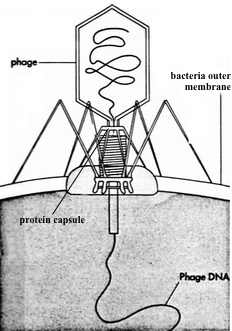
\includegraphics[width=0.4\textwidth]{figure1.png}
	\caption{A bacteriophage injecting its genome into a bacteria. The protein capsule both protects the 		genetic information while between hosts and pierces the membrane to allow injection.}
\end{figure}
Once the genome has gained entry to the bacteria, the virus hijacks the machinery the host uses to replicate its own genome. It also uses the host's ribosomes to synthesize proteins to promote its virulence as well as new proteins to encapsulate its copies. One of the last proteins made is lysozyme, which breaks open the bacterial cell membrane, killing the host and allowing many new copies of the virus to escape and spread to nearby cells.

Because the success of the virus means the death of the host, bacteria have evolved methods of resisting viruses. Coevolution has led to an arms race between viruses and bacteria, as they constantly find new ways to get around each other.

\section{Methods}
or Setup? How is our algorithm structured? Representation? What did we change from our inspiration?
soooo many fitnesses

\section{Results}
What are some things we've observed?

\section{Discussion}
What was hard? How close did we come to what other paper saw? What was new? What are some new directions to try? 

\section{Works Cited}
Pal, C., M.D. Marcia, A. Oliver, I. Schachar, and A. Buckling. 2007. Coevolution with viruses drives the \\\-\hspace{0.75cm} evolution of bacterial mutation rates. Nature Letters. 450: 1079-1081.

Todar, K. 2012. Bacteriophage. Online Textbook of Bacteriology. Accessed 6.4.2015.\\ \-\hspace{0.75cm} http://textbookofbacteriology.net/phage.html

\end{document}  